\documentclass[../main.tex]{subfiles}

\begin{document}
\chapter{Rozwiązywanie równania renderingu}

\section{Wstęp}

Wyprowadzone w poprzednim rozdziale równanie renderingu opisuje wszystkie badane przez nas efekty radiometryczne. Można je zapisać we wspomnianej już wcześniej formie całkowej:
\[
  L(\omega_o) = \int_{\Omega} {
      f_r(\omega_i, \omega_o)
      L_i(\omega_i)
      (n \cdot \omega_i)
      \dd{\omega_i}
  }
\]

W przypadku świateł zajmujących ciągły fragment dziedziny sferycznej, nie jesteśmy w stanie bezpośrednio przedstawić całki w postaci sumy skończonej bez znacznej utraty dokładności. Niestety, również dla większości funkcji $L_i$, $f_r$ rozwiązanie nie jest możliwe do znalezienia metodą analityczną w bardzo ograniczonym czasie wymaganym do zachowania płynności aplikacji.

Metody stosujące numeryczne podejście do wyznaczenia przybliżenia wartości tej całki będą opisane w kolejnych podrozdziałach. Wiedza na temat uzyskania przybliżenia oryginalnej całki przyda nam się do zrozumienia metod nie wymagających obliczenia pełnej całki równania renderingu oraz weryfikacji ich poprawności.

\section{Metoda Monte Carlo}

W ogólności całkowanie numeryczne funkcji nie jest możliwe do zrealizowania tak, aby błąd był niewielki przy relatywnie niskim czasie obliczeń, wystarczającym do uzyskania płynności działania. Jedną z szybszych metod całkowania numerycznego jest przybliżona metoda Monte Carlo, która bazuje na rachunku prawdopodobieństwa i prawie wielkich liczb. Metoda ta jest dokładnie opisana w publikacjach \cite{Sierocinski,MonteCarloAnderson,Veach}. W tym podrozdziale przytoczę podstawowe pojęcia i własności elementów ze statystyki matematycznej.

Zdarzeniem elementarnym nazywamy każdy możliwy wynik pewnego doświadczenia. Każde zdarzenie jest unikalne oraz dwa zdarzenia elementarne nie mogą wystąpić w trakcie jednego eksperymentu.

Zmienną losową $\mathbb{X}$ nazywamy funkcję przypisującą zdarzeniom elementarnym liczby. Przykładem zmiennej losowej jest liczba wylosowanych oczek na kostce, waga człowieka lub wzrost. Dziedzina zmiennej losowej może być dyskretna (np. liczba oczek na kostce tj. zbiór $\{1,2,3,4,5,6\}$) lub ciągła (np. przedział $[0,1]$). Wartość $Y = f(\mathbb{X})$, gdzie $f$ jest dowolną funkcją również jest zmienną losową. 

Funkcją rozkładu prawdopodobieństwa $P$ nazywamy funkcję przypisującą prawdopodobieństwo wartościom zmiennej losowej. 
% Jak to się ma dla zmiennych losowych ciągłych?

Dystrybuanta (ang. \textit{cumulative distribution function}, \textit{CDF}) wyznacza prawdopodobieństwo, że zdarzenie losowe $\mathbb{X}$, które zachodzi, ma wartość $\eta$ nie przekraczającą $x$.
\[
    F(x) = P(\mathbb{X} \leq x)
\]

Funkcją gęstości prawdopodobieństwa $f_{\mathbb{X}}$ (ang. \textit{probability density function}, \textit{PDF}) nazywamy pochodną dystrybuanty:
\[
    f_{\mathbb{X}}(x) = \frac{\dd F}{\dd x}(x)
\]

Wartości funkcji gęstości prawdopodobieństwa muszą być nieujemne oraz całka po całej dziedzinie zmiennej losowej $\Omega$ musi być równa $1$:
\[
    \int_{\Omega} f_{\mathbb{X}}(x) \dd x = 1
\]

Dla zmiennej losowej określonej na pewnym przedziale $\Lambda \in \mathbb{R}$ tż. $[a,b] \in \Lambda$ mamy:
\[
    \int_{a}^{b} f_{\mathbb{X}}(x) \dd x = P(a \leq x \leq b)
\]

Weżmy funkcję gęstości prawdopobieństwa $f_{\mathbb{X}}$ ciągłej zmiennej losowej $\mathbb{X}$. Wartość oczekiwana funkcji $g$ na ciągłej zmiennej losowej $\mathbb{X}$ wynosi:
\[
\mathbb{E}\left[ g(x) \right] =
\int_{\Omega}{
	g(x) f_{\mathbb{X}}(x)
	\: \dd x
}
\]

Wartość oczekiwaną możemy interpretować jako średnią wartość funkcji $g$, której parametry są wybierane zgodnie z rozkładem reprezentowanym przez $f$.

Wariancją nazywamy funkcję wyznaczającą kwadrat oczekiwanych odchyleń od wartości oczekiwanej. Wariancja $V$ funkcji $g$ zdefiniowana jest intuicyjnie jako:
\[
V\left[ g(x) \right] 
	=
	\mathbb{E}\left[ 
		\left( 
			g(x) - \mathbb{E}\left[ g(x) \right] 
		\right)^2 
	\right]
	=
	\mathbb{E}\left[
		f(x)^2
	\right] - \mathbb{E}\left[
		f(x)
	\right]^2
\]

Własności wartości oczekiwanej i wariancji:
\begin{gather*}
\mathbb{E}\left[ag(x)\right] = a \mathbb{E} \left[g(x)\right] \\
\mathbb{E}\left[\sum_{i} g(x_i)\right] = \sum_{i} \mathbb{E} \left[g(x_i)\right] \\
V\left[ ag(x) \right] = a^2 V\left[g(x)\right]
\end{gather*}

Jeżeli zmienne losowe $\mathbb{X}_i$ są niezależne, to również zachodzi:
\[
\sum_{i} V \left[
	g(\mathbb{X}_i)
\right]
=
V \left[
	\sum_{i} g(\mathbb{X}_i)
\right]
\]

Estymatorem Monte Carlo przybliżającym wartość $\mathbb{E}(g(x))$ opartym na prawie wielkich liczb nazywamy:
\[
\widetilde{g_n}(x) =
	\frac{1}{n}
	\sum_{i=1}^{n}g(x_i)
\]

\noindent gdzie $x=(x_1, \ldots, x_n)$ jest zbiorem $n$ próbek zmiennej losowej $\mathbb{X}$.

\section{Generowanie próbek}

Próbki Monte-Carlo można wybierać w sposób całkowicie losowy, jednak taka metoda nie daje nam żadnej gwarancji, że wybrane próbki będą pokrywały dziedzinę w sposób równomierny, co łatwo zaobserwować na rys. \ref{fig:RandomSamples}. Z pomocą przychodzą nam ciągi \textit{quasi-losowe}, które pokrywają zadaną dziedzinę w sposób, który gwarantuje nam jednorodne pokrycie dziedziny. Załóżmy, że nasza dziedzina jest kostką $n$-wymiarową $[0,1]^{n}$.

\begin{figure}[h]
  \centering
  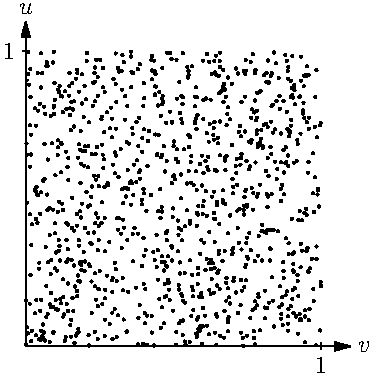
\includegraphics[height=5cm]{montecarlo/random_seq.pdf}
  \caption{Próbki wygenerowane w sposób losowy (1024 próbek). Opracowanie własne.}
  \label{fig:RandomSamples}
\end{figure}

Pierwszą metodą jednorodną (rys. \ref{fig:UniformSamples}) jaka się narzuca jest zbudowanie równomiernej siatki posiadającej $m$ punktów na boku kostki. Problemem tej metody jest jej zbyt duża jednorodność, wybrane punkty są ułożone w bardzo precyzyjny sposób przez co pewne szczegóły szacowanej funkcji mogą zostać ominięte.

\begin{figure}[h]
  \centering
  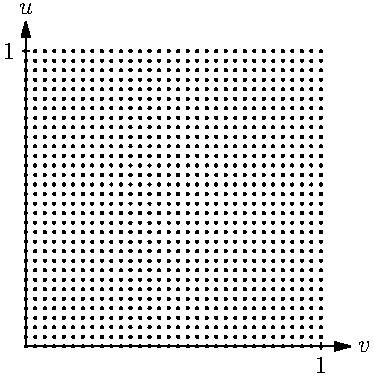
\includegraphics[height=5cm]{montecarlo/uniform_seq.pdf}
  \caption{Próbki wygenerowane przez równomierny podział (1024 próbek). Opracowanie własne.}
  \label{fig:UniformSamples}
\end{figure}

Ciągi o niskiej rozbieżności są rozwiązaniem tego problemu: są to ciągi deterministyczne, które na pierwszy rzut oka wydają się losowe przez co posiadają ich zalety oraz pokrywają równomiernie całą dziedzinę niezależnie od wybranej ilości punktów.

Najbardziej znanymi ciągami tego typu jest ciąg \textit{van der Corputa} oraz jego pochodne czyli ciąg Haltona, zbiór Hammersleya.

\subsection{Ciąg van der Corputa}

Ciąg van der Corputa \cite{WongSamplingWH} jest jednowymiarowym ciągiem o niskiej rozbieżności, zdefiniowanym na zbiorze $[0,1]$ zbudowanym poprzez odwrócenie bazy reprezentacji w danym systemie o podstawie $b$. Każda liczba całkowita $i$ może zostać przedstawiona w pewnej zadanej bazie w sposób następujący:
\[ 
i = \sum_{j=0}^{\infty} {a_j b^j} \quad \forall_{j}\: a_j < b
\]

Ciąg van der Corputa transformuje powyższą reprezentację (ciąg $a_k$), dla $n$-tego elementu otrzymujemy:
\[ 
v_b(n) = \sum_{j=0}^{\infty} {a_j b^{-j-1}} 
\]

\begin{example}
  Weźmy liczbę $7$ i bazę $2$. Reprezentacja tej liczby może zostać rozpisana jako (bez zer nieznaczących):
  \[ 
  7 = 1 * 2^0 + 1 * 2^1 + 1 * 2^2 = (111)_{b} 
  \]

  \noindent Zatem:
  \[
    v_{2}(7)
      = \frac{1}{2^{1}} + \frac{1}{2^{2}} + \frac{1}{2^{3}}
      = \frac{1}{2} + \frac{1}{4} + \frac{1}{8}
      = 0.875
      \in (0,1)
  \]
\end{example}

Warto zauważyć, że $\sum_{n=1}^{\infty} \frac{b-1}{b^n} = 1$ dla $b>1$.

Kod realizujący powyższe zadanie może być zapisany w formie:

\begin{lstlisting}[language=c++]
double VanDerCorput(unsigned int n, unsigned int base) {
  auto denominator = 1.0;
  auto result = 0.0;

  while (n > 0) {
    denominator /= base;
    result += denominator * (n % base)
    n /= base;
  }

  return result;
}
\end{lstlisting}

Istnieje alternatywne rozwiązanie korzystające z właściwości operacji takiej odwrotności. Warto zauważyć, że obie liczby $n$ oraz $v_b(n)$ zapisane w systemie o podstawie $b$ (tutaj $b=2$) są odbiciem lustrzanym:
\[
  5 = 1 + 4 = (101.0)_{b} \quad
  (0.101)_{b} = 0.625 = \frac{1}{2} + \frac{1}{8} = v_2(5)
\]

Dla $b=2$ odpowiednio skonstruowana operacja bitowa tego typu pozwoli na uzyskanie poprawnego wyniku i zwiększenie wydajności obliczeń \cite{dammertz_2012,MultidimensionalSampling}:

\begin{lstlisting}[language=c++]
double VanDerCorputRadicalInverse(unsigned int bits)
{
	bits = (bits << 16) | (bits >> 16);
	bits = ((bits & 0x00ff00ff) <<  8) | ((bits & 0xff00ff00) >>  8);
	bits = ((bits & 0x0f0f0f0f) <<  4) | ((bits & 0xf0f0f0f0) >>  4);
	bits = ((bits & 0x33333333) <<  2) | ((bits & 0xcccccccc) >>  2);
	bits = ((bits & 0x55555555) <<  1) | ((bits & 0xaaaaaaaa) >>  1);

	return (double) bits / (double) 0x100000000LL;
}
\end{lstlisting}

\subsection{Ciąg Haltona}

Ciąg Haltona jest uogólnieniem ciągu van der Corputa do wyższych wymiarów. Weźmy $n$ wzajemnie względnie pierwszych liczb $b_i$ większych od 1, czyli takiego zbioru w którym dla dowolnej pary liczb ich jedynym wspólnym dzielnikiem jest 1.

$i$-ty $n$-wymiarowy element ciągu Haltona równy jest:
\[ 
x(i) = \left( v_{b_1}(i), v_{b_2}(i), \cdots, v_{b_n}(i) \right) 
\]

\begin{figure}[h]
  \centering
  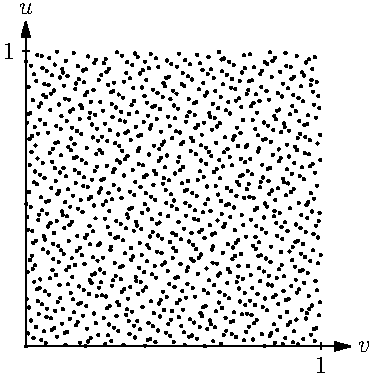
\includegraphics[height=5cm]{montecarlo/halton_seq.pdf}
  \caption{Ciąg Haltona dla $b_1=2$ i $b_2=3$ (1024 próbek). Opracowanie własne.}
  \label{fig:HaltonSamples}
\end{figure}

\subsection{Zbiór Hammersleya}

Zbiór Hammersleya jest ciągiem bardzo podobnym do ciągu Haltona, również korzystającym z ciągu van der Corputa. Chcemy wygenerować $m$ punktów, weźmy $n-1$ wzajemnie względnie pierwszych liczb $b_i$ większych od 1. $i$-tym $n$ wymiarowym elementem ciągu jest:
\[
  x(i) = \left(
    \frac{i}{m}, v_{b_1}(i), v_{b_2}(i), \cdots, v_{b_{n-1}}(i)
  \right)
\]

Warto zauważyć, że dla wielu zastosowań potrzebujemy jedynie dwuwymiarowej parametryzacji. W takim przypadku będziemy potrzebować jednego ciągu składowego van der Corputa, zatem bardzo wygodnie jest skorzystać z  z wersji bitowej do generowania liczb. Ten zbiór będzie wykorzystywany w kodzie pracy.

\begin{figure}[h]
  \centering
  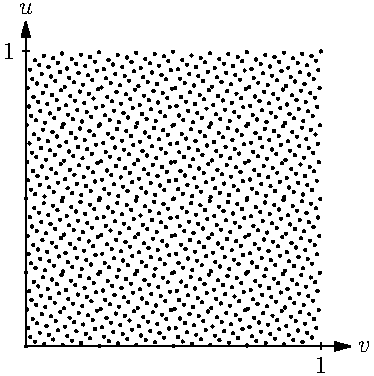
\includegraphics[height=5cm]{montecarlo/hammersley_seq.pdf}
  \caption{Zbiór Hammersleya dla $b_1=2$ (1024 próbek). Opracowanie własne.}
  \label{fig:HammersleySamples}
\end{figure}

\subsection{Generowanie próbki z funkcji gęstości prawdopodobieństwa metodą inwersji}
\label{section:pdfsampling}

Weźmy funkcję gęstości prawdopodobieństwa $f(x)$. Jej dystrybuanta jest równa:
\[ 
F(s_x) = \int_{-\infty}^{s_{x}} f(x) dx \in [0,1] 
\]

Załóżmy, że mamy do dyspozycji parametr $\xi \in [0,1]$ wygenerowany dowolną metodą. Zbudujmy równanie w którym niewiadomą będzie $s_x$:
\[ 
F(s_x) = \xi
\]

Rozwiązując powyższe równanie dla $s_x$ otrzymamy funkcję odwrotną generującą próbkę $s_x$:
\[
s_x = F^{-1}(\xi)
\]

Dla niektórych funkcji, nie omawianych w tej pracy, obliczenie wartości całki lub znalezienie rozwiązania może nie być możliwe. Istnieją jednak inne metody próbkowania takich funkcji: metoda odrzucania (ang. \textit{rejection method}) oraz transformacja Boxa-Mullera \cite{pbrt}.

\subsection{Generowanie punktów na półsferze}

Generowanie punktów na półsferze jest bardzo ważnym zagadnieniem związanym z wykorzystaniem metody Monte-Carlo. Próbkowanie równania renderingu wymaga wyznaczenia zbioru testowych kierunków padania światła. Najczęściej, wszystkie możliwe kierunki przychodzące oraz wychodzące promieni znajdują się w obszarze półsfery zdefiniowanej przez punkt oraz normalną do symulowanej powierzchni w tym punkcie. Mając, więc metodę generowania równomiernego zbioru punktów na sferze będziemy znać sposób wyznaczania kierunków.

Do wygenerowania punktów na półsferze możemy wykorzystamy parametryzację z kostki dwuwymiarowej do współrzędnych sferycznych:
\[
  (u,v) \in [0,1]^2 \rightarrow (\theta, \phi) \in \mathcal{H}
\]

Parametry wejściowe $(u,v)$ wygenerujemy za pomocą ciągów pseudolosowych przedstawionych wcześniej. Obrazki poglądowe wykorzystują ciąg Hammersleya jako generator liczb wejściowych.

Niestety, proste przeskalowanie dziedziny źródłowej tzn. przekształcenie parametrów przekształceniem liniowym postaci:
\begin{align*}
	\phi &= \frac{1}{2} \pi u \\
 	\theta &= 2 \pi v
\end{align*}
\noindent nie będzie wystarczające, ponieważ otrzymany rozkład nie będzie równomierny na powierzchni półsfery (więcej punktów jest skupionych w okolicach biegunów, rys. \ref{fig:SpherePointsNaive}) \cite{WolframSpherePointPicking}.

\begin{figure}[h]
    \centering
    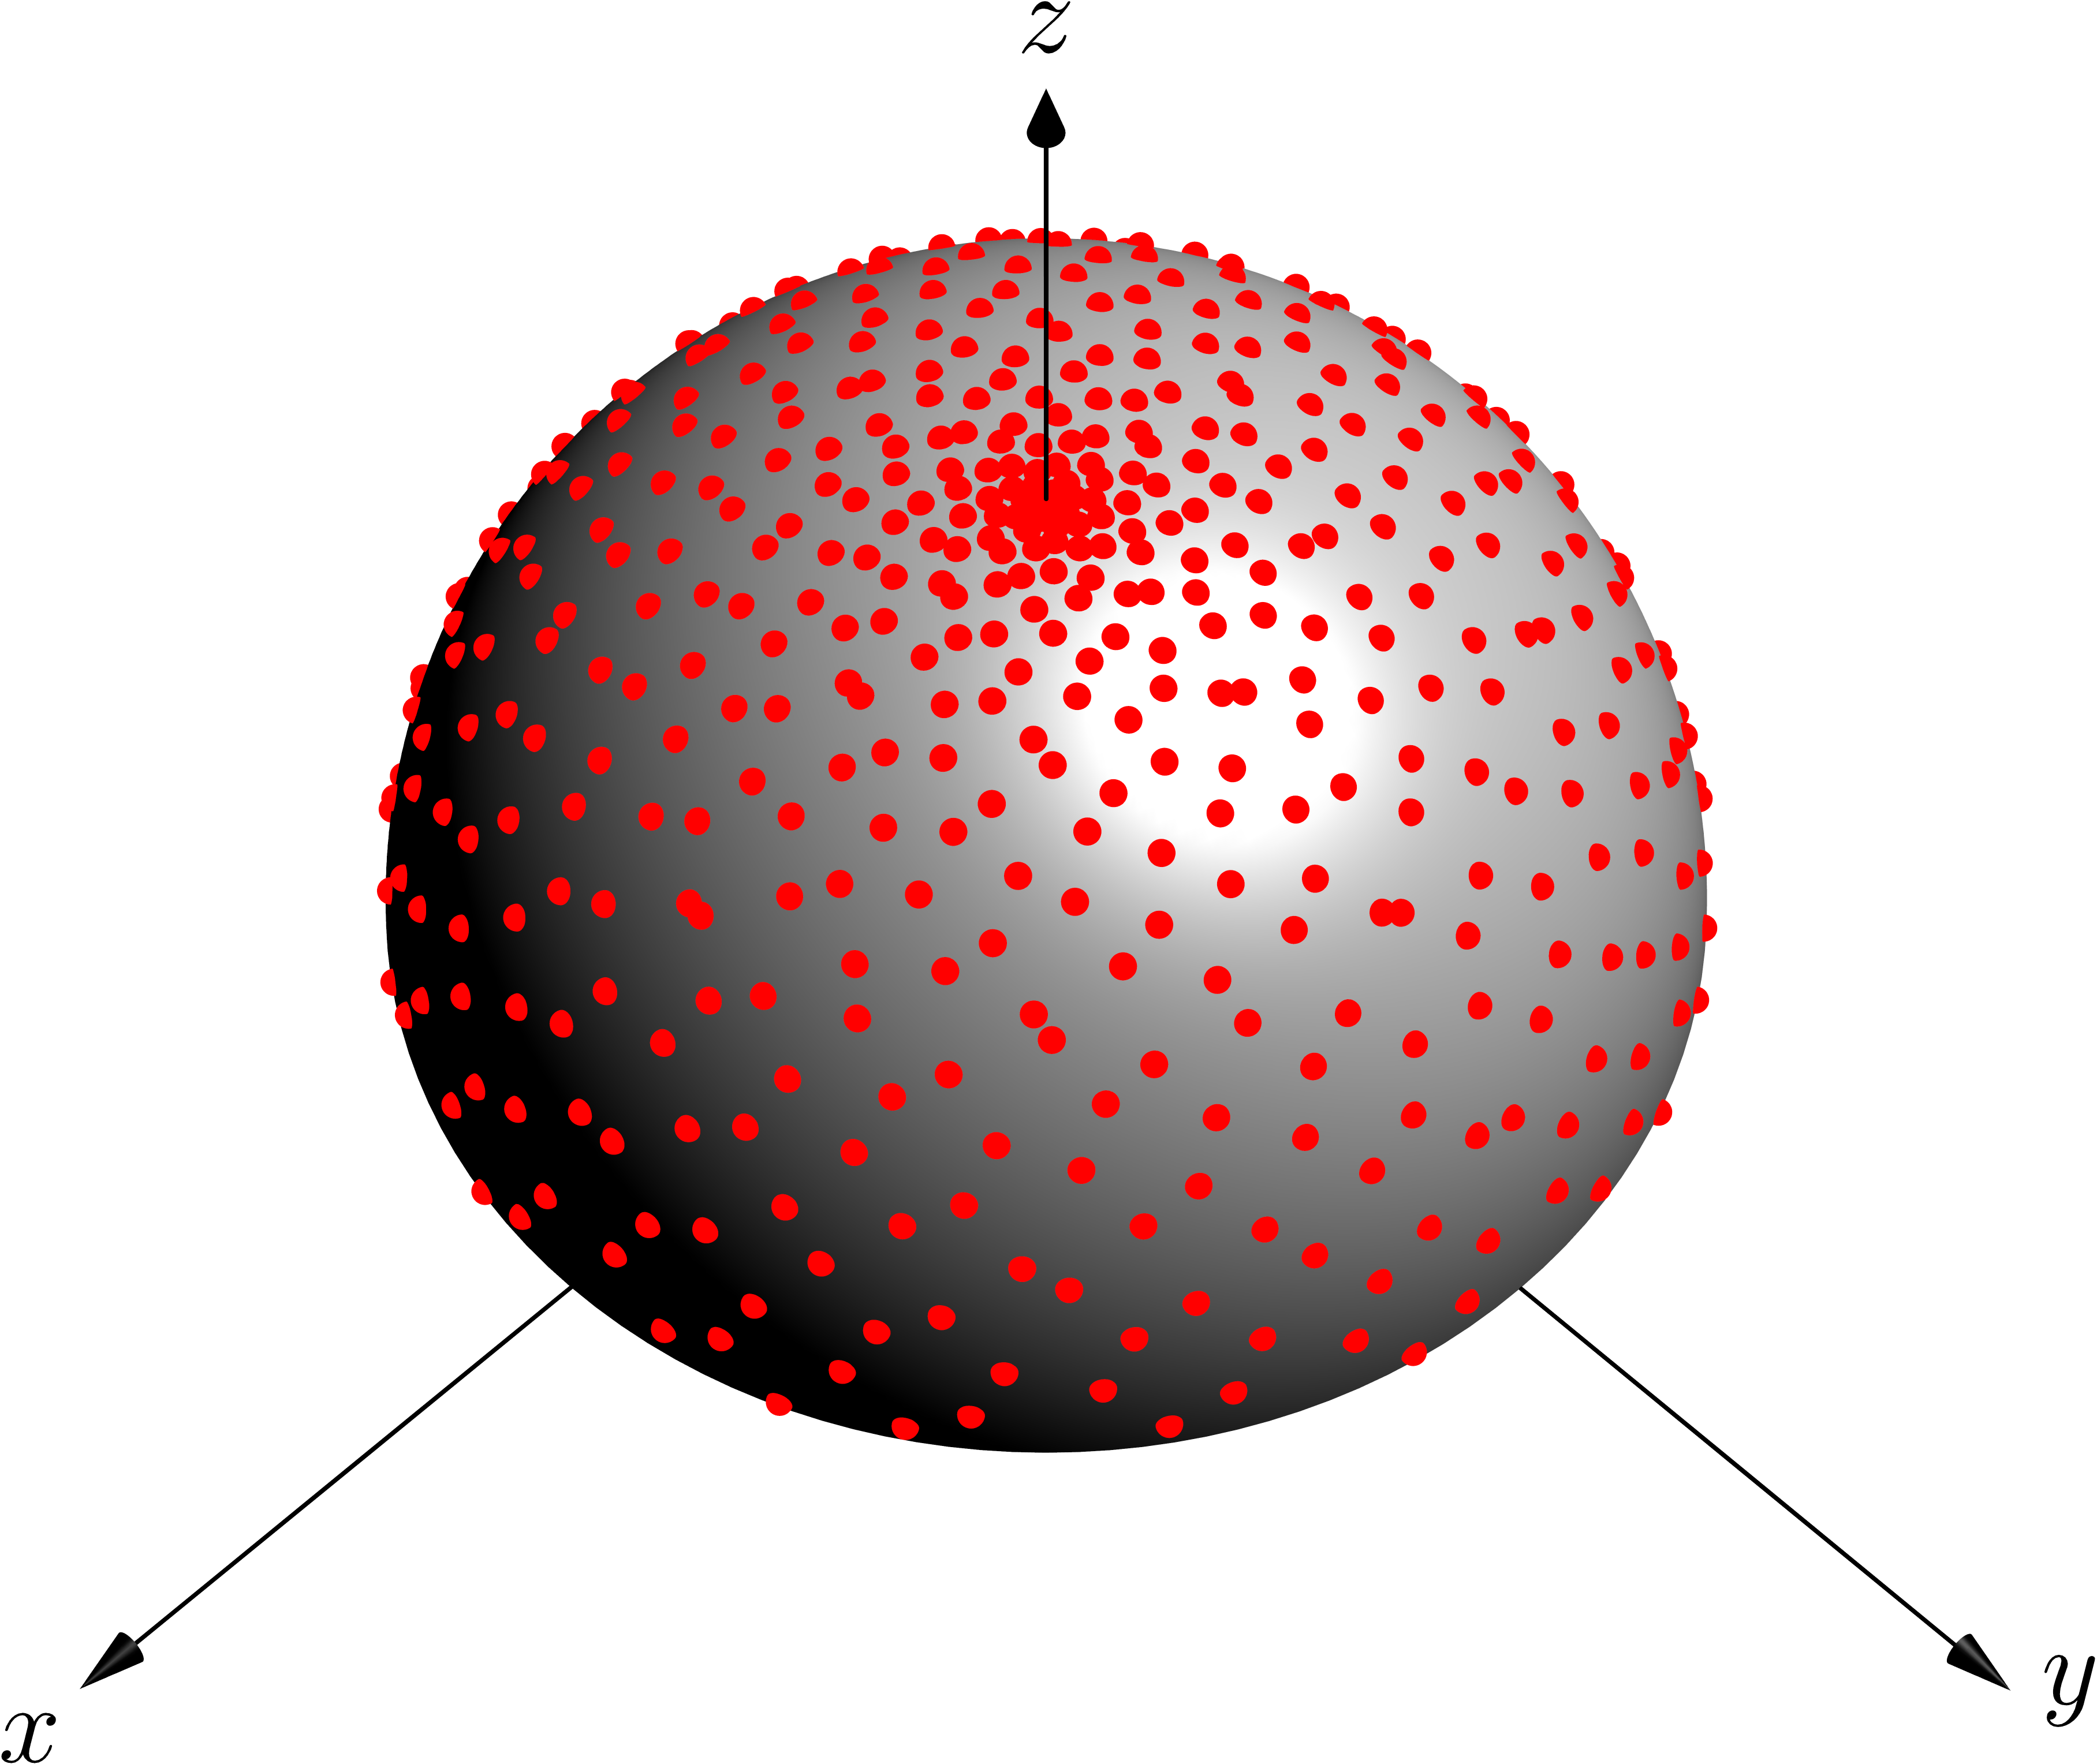
\includegraphics[height=6cm]{montecarlo/sphere_points_naive.png}
    \caption{Punkty na sferze wygenerowane metodą naiwną (500 próbek). Opracowanie własne.}
    \label{fig:SpherePointsNaive}
\end{figure}

Alternatywne rozwiązanie znajdziemy stosując metodę przedstawioną w sekcji \ref{section:pdfsampling}  przy założeniu, że funkcja gęstości prawdopodobieństwa jest stała \cite{dammertz_2012, AdvancedCGRenderingEq}:
\begin{align*}
	\phi &= \cos^{-1}(1-u) \\
	\theta &= 2 \pi v
\end{align*}

Na rysunku \ref{fig:SpherePointsUniform} wyraźnie widać, że punkty przestały być skupione wokół bieguna.

\begin{figure}[h]
    \centering
    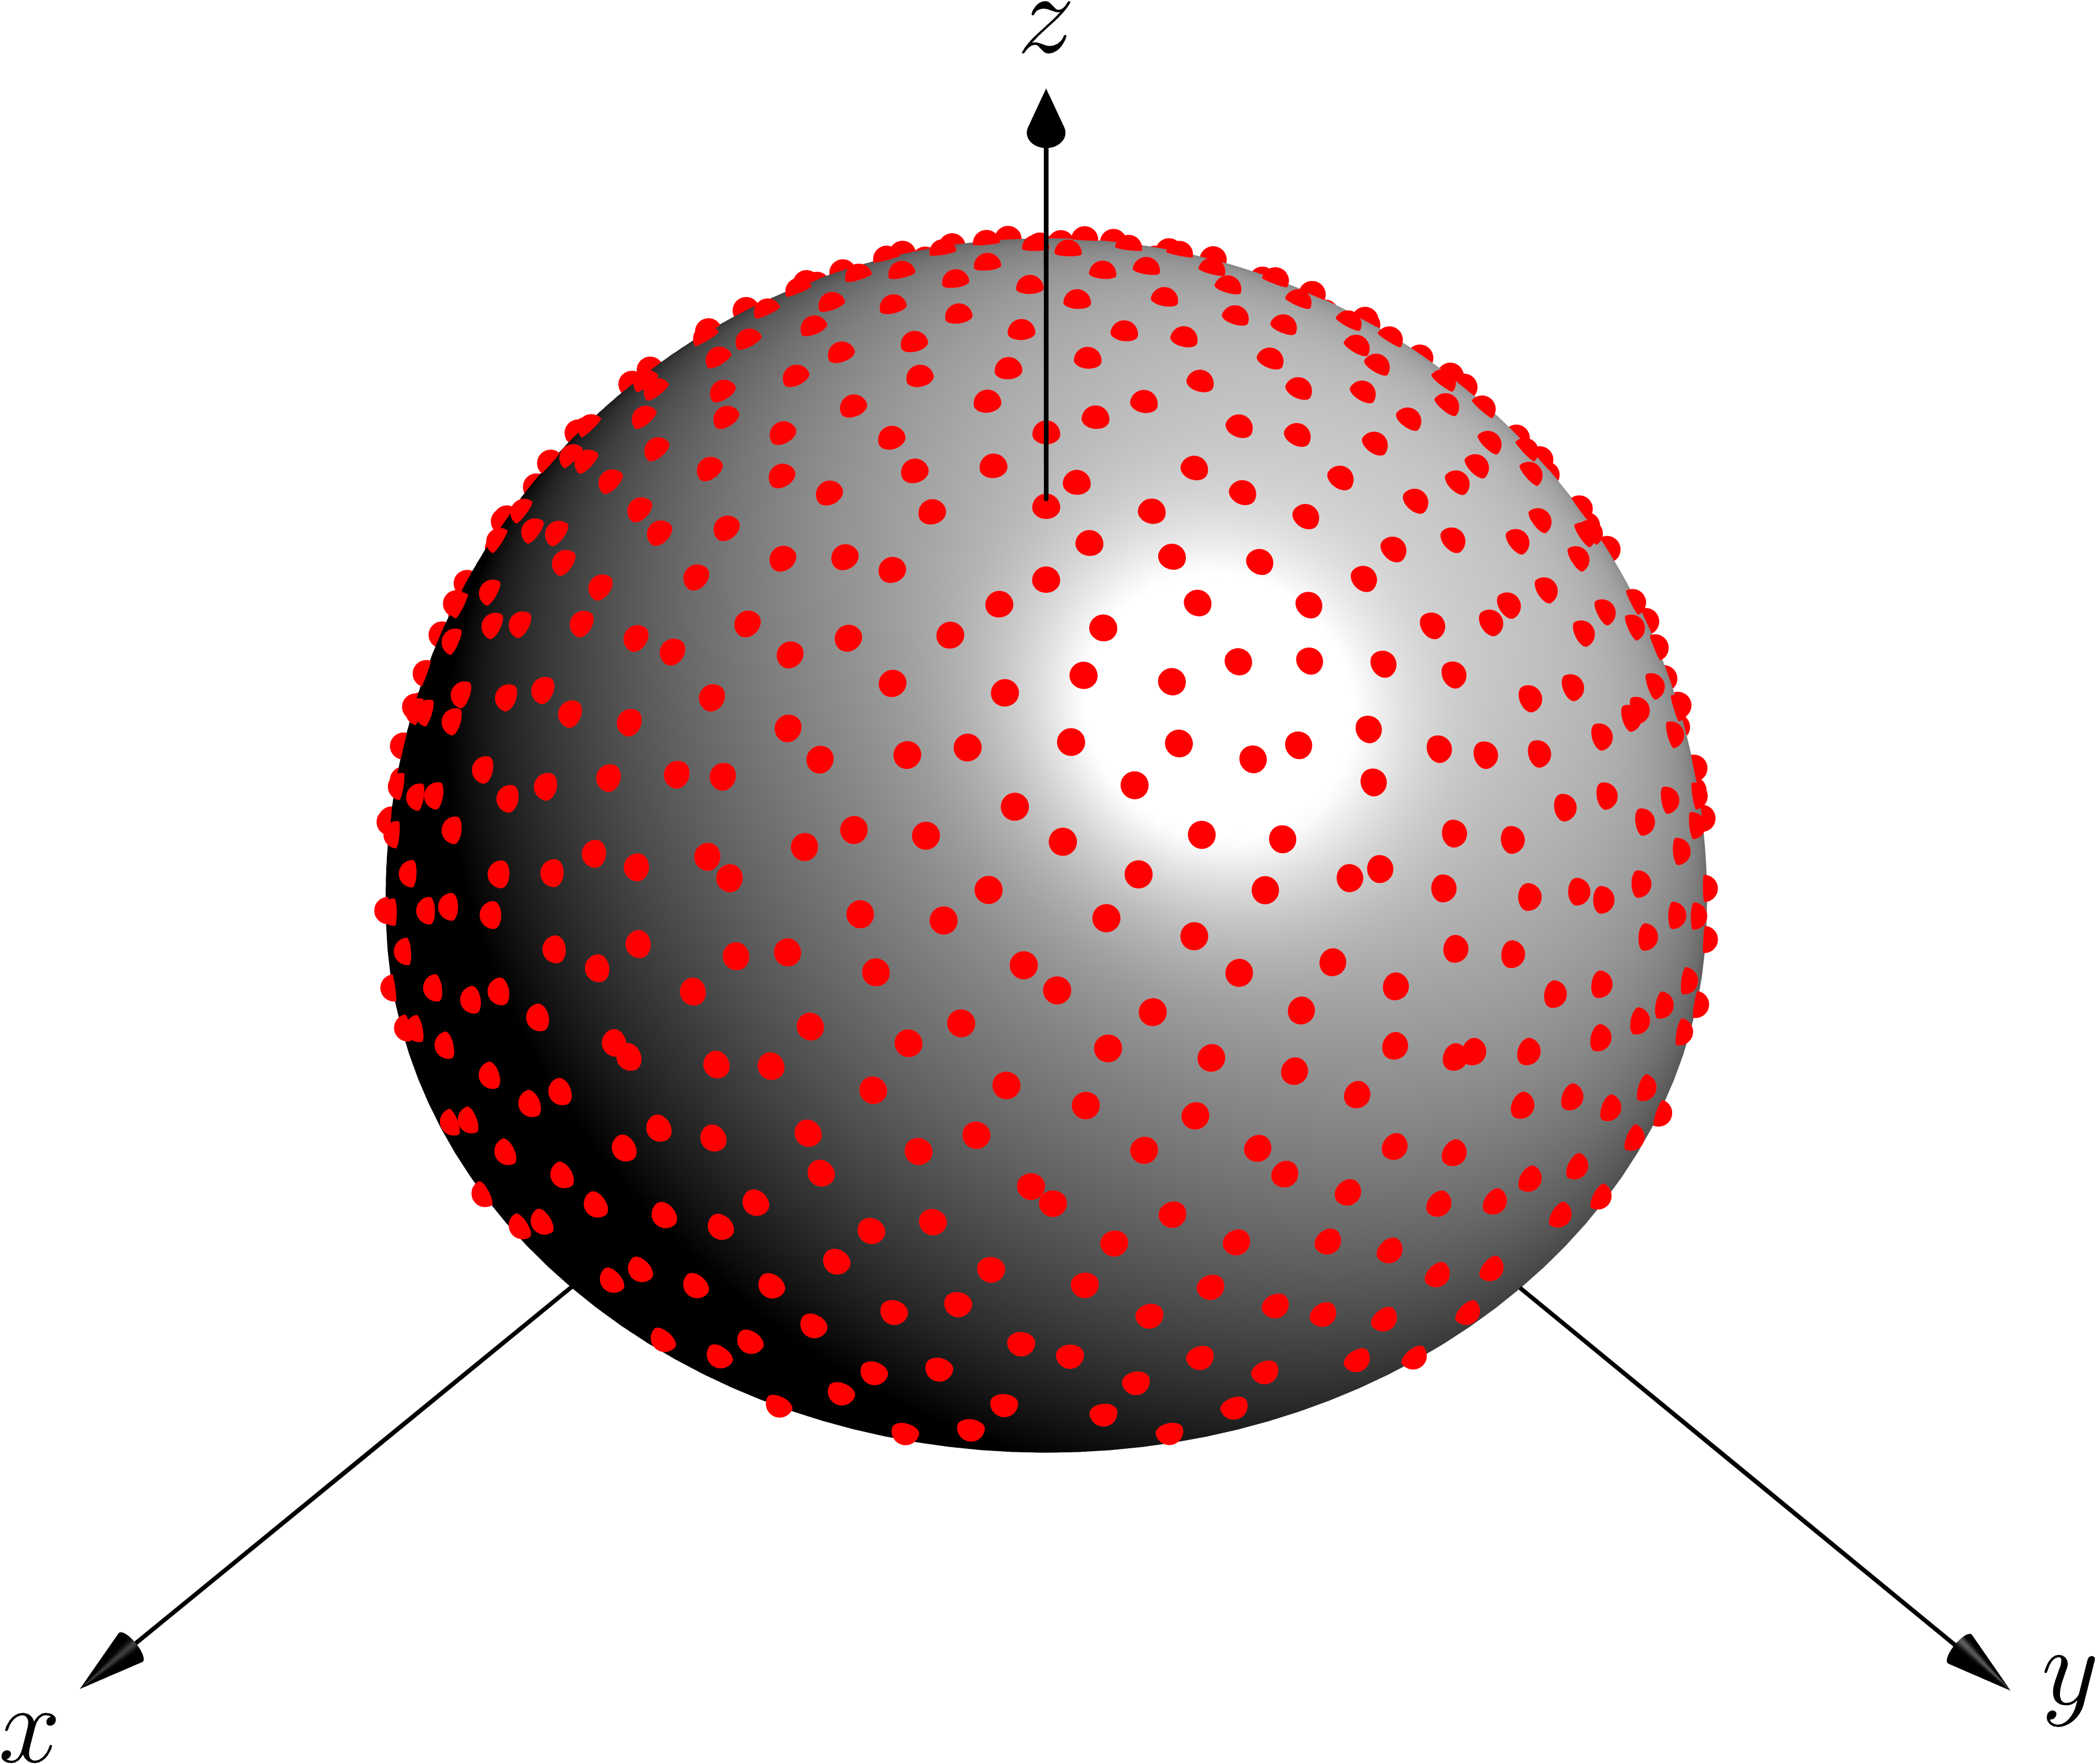
\includegraphics[height=6cm]{montecarlo/sphere_points_uniform.png}
    \caption{Punkty na sferze wygenerowane metodą inwersji (500 próbek). Opracowanie własne.}
    \label{fig:SpherePointsUniform}
\end{figure}

Dla funkcji które są zależą od kosinusa kąta $\phi$ możemy wykorzystać alternatywną metodę generowania, która będzie generować mniej punktów w okolicach horyzontu (rys. \ref{fig:SpherePointsCosine}), gdzie $\cos\phi \approx 0$. Do wyznaczenia takiego rozkładu wykorzystamy funkcję gęstości prawdopodobieństwa $p$ proporcjonalną do czynnika $\cos \phi$, finalnie otrzymamy \cite{AdvancedCGRenderingEq}:
\begin{align*}
  \phi &= \cos^{-1}(\sqrt{1-u}) \\
  \theta &= 2 \pi v
\end{align*}

\begin{figure}[h]
    \centering
    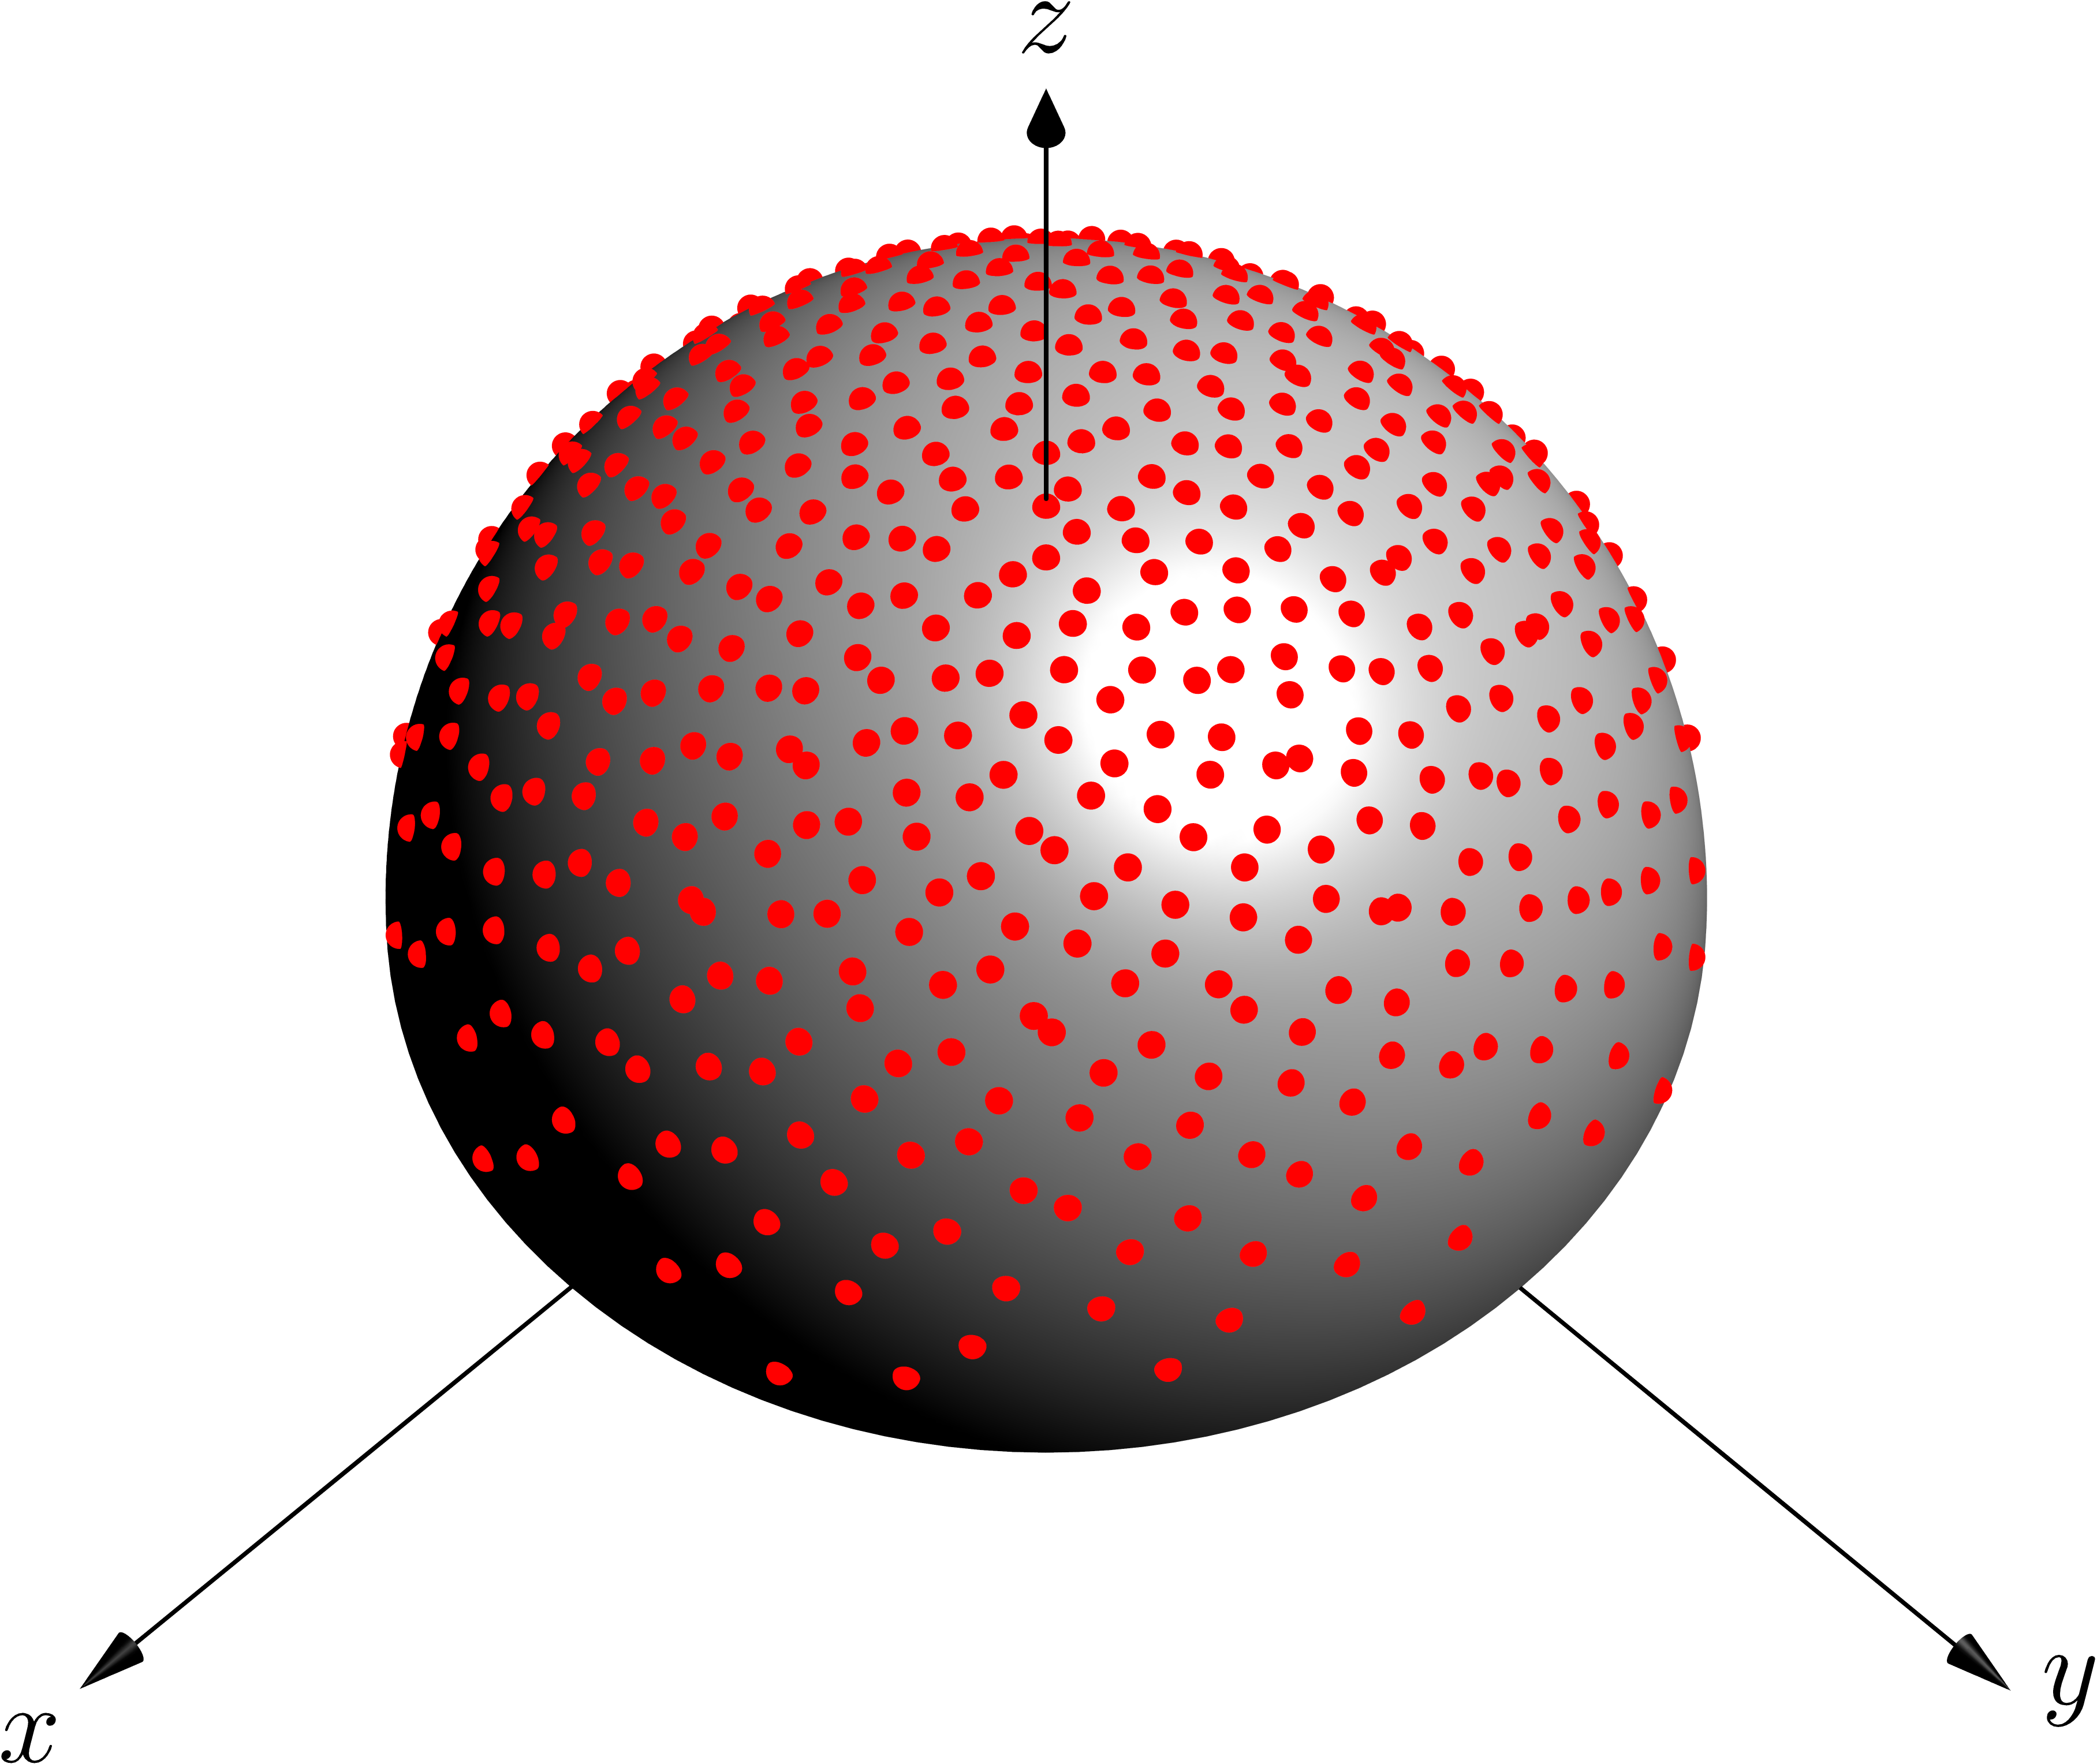
\includegraphics[height=6cm]{montecarlo/sphere_points_cosine.png}
    \caption{Punkty na sferze wygenerowane metodą inwersji z uwzględnieniem czynnika $\cos\phi$ (500 próbek). Opracowanie własne.}
    \label{fig:SpherePointsCosine}
\end{figure}

\section{Przyrostowa metoda Monte-Carlo}

Metoda Monte-Carlo ze względu na swoją złożoność obliczeniową nie umożliwia uzyskania rezultatu w czasie rzeczywistym. Możliwość operowania sceną, precyzyjnego ustawienia kamery i obiektów nie jest łatwe w takim środowisku. Często nie potrzebujemy również bardzo dużej szczegółowości - w niektórych przypadkach wystarczy nam konkretna ilość iteracji do znalezienia problemu obecnej implementacji lub oceny głównych różnic między metodami.

Wygodnym kompromisem jest podzielenie obliczeń na wiele etapów, z których każdy może zostać wyświetlony jako częściowy podgląd. Dłuższy czas oczekiwania bez zmian w scenie pozwala nam uzyskać większą jakość.

Spróbujmy zbudować rekurencyjny ciąg podsum Monte-Carlo wyznaczających wynik dla $n$-tej próbki oraz po dołączeniu $n+1$ próbki:
\begin{align*}
I_n &= \frac{1}{n} \sum_{i=1}^{n} f(x_i) \\
I_{n+1} &= \frac{1}{n+1} \sum_{i=1}^{n+1}f(x_i) \\
	&= \frac{n}{(n+1)n} \sum_{i=1}^{n}f(x_i) + \frac{1}{n+1}f(x_{n+1}) \\
	&= \frac{n}{n+1} I_{n} + \frac{1}{n+1}f(x_{n+1})
\end{align*}

Dodatkowy czas potrzebny na przygotowanie ramki, policzenie sumy ważonej i wyświetlenie rezultatu na ekranie sprawia, że uzyskamy szybszą zbieżność przez zgrupowanie próbkek w pakiety, które mogą zostać potencjalnie policzone jednocześnie. Okazuje się, że rozpisanie analogicznego równania dla paczek danego, stałego rozmiaru jest trywialne:
\begin{align*}
  I_{(m+1)n} &= \frac{1}{(m+1)n} \sum_{i=1}^{(m+1)n} f(x_i)
  = \frac{1}{(m+1)n} \sum_{i=1}^{mn} f(x_i)
    + \frac{1}{(m+1)n} \sum_{i=mn+1}^{(m+1)n} f(x_i) = \\
  &= \frac{m}{(m+1)mn} \sum_{i=1}^{mn} f(x_i)
    + \frac{1}{(m+1)n} \sum_{i=mn+1}^{(m+1)n} f(x_i) \\
  &= \frac{m}{m+1}I_{mn}
    + \frac{1}{m+1} \left(
        \frac{1}{n} \sum_{i=mn+1}^{(m+1)n} f(x_i)
    \right)
\end{align*}

Powyższe obliczenie sumy ważonej może zostać zrealizowane za pomocą łańcucha buforów ramki i obliczone za pomocą wspartego sprzętowo mechanizmu łączenia kolorów (ang. \textit{blending}). Obecna partia musi być liczona w osobnym buforze oraz potem skopiowana do docelowego z wykorzystaniem mieszania. Można zastosować uproszczenie, w którym wykorzystamy tylko jeden bufor, ale często ze względu na istnienie wielu świateł i wybraną technikę np. odroczone cieniowanie (ang. \textit{deferred shading}) może być koniecznie zastosowanie przynajmniej dwóch.

\section{Metoda funkcji ważności}

Metoda funkcji ważności (ang. \textit{importance sampling}) jest jedną z metod ograniczania wariancji metody Monte-Carlo. Innymi słowy, zastosowanie tej techniki poprawnie powinno skrócić czas w którym ciąg zbiegnie do odpowiednio bliskiej wartości całki.

Publikacje \cite{Veach,MonteCarloAnderson} sugerują zastosowanie innej techniki generowania próbek tak, aby znacznie częściej wybierać próbki istotne dla wyniku.

Mając funkcję gęstości $h(x)$ zmiennej losowej $\mathbb{X}$ na której potrafimy całkować, wyznaczać jej wartość w punkcie oraz jest prawie proporcjonalna do całkowanej funkcji $g(x)$ możemy przepisać:
\[
  \int_{x \in \mathbb{A}} { g(x) dx } =
  \int_{x \in \mathbb{A}} { g(x) \frac{h(x)}{h(x)} dx } =
  \int_{x \in \mathbb{A}} { \frac{g(x)}{h(x)} h(x) dx } =
  \mathbb{E}_{h}\left({ \frac{g(x)}{h(x)} }\right)
\]

Jeżeli funkcja gęstości prawdopodobieństwa $h(x)$ zostanie wybrana w odpowiedni sposób to wariancja estymatora Monte-Carlo zmniejszy się. Aby funkcja $h(x)$ była użyteczna, musi spełniać kilka warunków:

\begin{itemize}

  \item obliczenia dotyczące funkcji $h$ muszą być łatwo realizowalne, obliczenie wartości funkcji, jej całki musi być możliwe bez wykorzystania metody Monte-Carlo,

  \item symulowanie próbek z rozkładu $h$ musi być realizowalne,

  \item $h(x) > 0$ dla $g(x) \neq 0$,

  \item $h(x)$ musi być możliwie proporcjonalne do $|g(x)|$, inaczej wariancja zamiast zmaleć, wzrośnie.

\end{itemize}

Teoretycznie najlepszym wyborem jest funkcja $g'(x) = cg(x)$, gdzie:
\[
	c \propto \frac{1}{\int_{\Omega}{g(x)dx}}
\]

\noindent Niestety, taka funkcja jest niemożliwa do wykorzystania praktycznego w sposób bezpośredni, ponieważ mianownik w stałej $c$ jest naszą szukaną całką, której przecież nie potrafimy policzyć. Będziemy szukać funkcji $h$ podobnych kształtem do $g$.

Istotnym problemem tej metody jest to, że nieuważny wybór funkcji $h$ może znacząco pogorszyć wariancję (rys. \ref{fig:ImportanceSamplingProblems}).

\begin{figure}
  \centering

  \begin{subfigure}[t]{0.45\textwidth}
    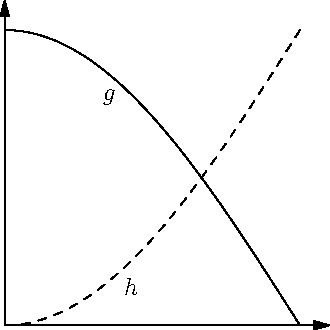
\includegraphics[width=\textwidth]{montecarlo/different_shape}
    \label{fig:ImportanceSamplingWrongFunction}
    \caption{$h$ nie odwzorowuje kształtu funkcji $g$}
  \end{subfigure}
  \begin{subfigure}[t]{0.45\textwidth}
    \centering
    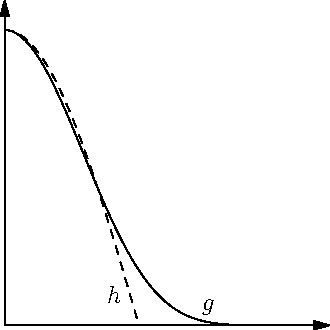
\includegraphics[width=\textwidth]{montecarlo/lost_tail}
    \label{fig:ImportanceSamplingLostTail}
    \caption{$h$ nie obejmuje ogona rozkładu funkcji $g$}
  \end{subfigure}

  \caption{Przykłady problemów związanych z wyborem $h(x)$. Opracowanie własne.}
  \label{fig:ImportanceSamplingProblems}
\end{figure}

\section{Funkcja ważności dla poszczególnych rodzajów BRDF}

Pozostaje jeszcze kwestia znalezienia konkretnej funkcji $h(x)$ z której będziemy mogli skorzystać przy zastosowaniu metody funkcji ważności. Po pierwsze, funkcja $h(x)$ musi mieć podobny kształt do funkcji podcałkowej oraz musimy potrafić wygenerować próbkę.

\subsection{Phong BRDF}

Znajdźmy funkcję gęstości prawdopodobieństwa nadającą się do generowania próbek dla BRDF Phonga \cite{NotesImportanceSampling,ImportanceSamplingForProduction}:
\[
  L_o(\omega_o) = \int_{\Omega} {
    L_i(\omega_i) \cos^{n}\theta_s \cos\theta_i \dd \omega_i
  }
\]

Będziemy poszukiwać funkcji $p(\theta, \phi)$ z której będziemy mogli wygenerować próbki korzystając z funkcji odwrotnych:
\begin{align*}
  s_\theta &= F_{\theta}^{-1}(\xi_\theta) \\
  s_\phi &= F_{\phi}^{-1}(\xi_\phi)
\end{align*}

\noindent użytecznych do oszacowania całki:

Interesuje nas odwzorowanie kształtu części $\cos^{n}\theta_s$ w odniesieniu do kąta bryłowego $\dd \omega_i$. Wykorzystajmy tą funkcję jako kształt dla szukanej funkcji gęstości prawdopodobieństwa. Funkcja gęstości $p(x)$ musi spełniać warunek:
\[ 
\int_{-\infty}^{\infty} p(x) \dd x = 1 
\]

\noindent stąd (czynnik $\sin\theta$ pochodzi z zamiany do współrzędnych sferycznych z kątów bryłowych):
\[
  p(\theta, \phi) = \frac{
    \cos^{n}{\theta} \sin\theta
  }{
    \int_{0}^{2\pi} \int_{0}^{\frac{\pi}{2}} {
      \cos^{n}{\theta} \sin\theta \dd \theta
    }
  }
\]

Rozwiązując poniższą całkę otrzymujemy poniższy dwuwymiarowy rozkład gęstości prawdopodobieństwa (patrz listing \ref{appendix:maxima_phong}):
\[
  p(\theta, \phi) =
    \frac{n+1}{2\pi} \cos^{n}\theta \sin\theta
\]

Rozbijmy zmienne $\theta$ oraz $\phi$ na dwie oddzielne niezależne funkcje korzystając z rozkładu brzegowego (ang. \textit{marginal density function}):
\[
  p(\theta) = \int_{0}^{2\pi} {
    p(\theta, \phi) \dd \theta
  } =
  (n+1) \cos^{n}{\theta} \sin\theta
\]

Korzystając z twierdzenie Bayesa możemy obliczyć rozkład warunkowy $p(\phi | \theta)$:
\[
  p(\phi | \theta) = \frac{
    p(\theta, \phi)
	}{
		p(\theta)
	} = \frac{1}{2\pi}
\]

Oba rozkłady konwertujemy do postaci dystrybuanty którą będziemy próbkować korzystając ze zmiennych losowych $(\xi_{\theta}, \xi_{\phi}) \in [0,1]^2$:
\[
	\xi_\phi = P(s_{\phi}) =
	\int_{0}^{s_{\phi}} {
		p(\phi) \dd \phi
	} =
	\int_{0}^{s_{\phi}} {
		\frac{1}{2\pi} \dd \phi
	} =
	\frac{s_{\phi}}{2\pi}
\]

Stąd możemy wyznaczyć:
\[
	s_{\phi} = 2 \pi \xi_{\phi}
\]

Analogicznie postępujemy z rozkładem brzegowym:
\[
  \xi_{\theta} = P(s_{\theta}) =
	\int_{0}^{s_{\theta}} {
		p(\theta) \dd \theta
	} =
	\int_{0}^{s_{\theta}} {
		\frac{n+1}{2\pi} \cos^{n}\theta \sin\theta \dd\phi
	} =
	1 - \cos^{n+1}(s_{\theta})
\]

Z czego mamy:
\[
	s_{\theta} =
	\cos^{-1}\left[
		(1 - \xi_{\theta})^{\frac{1}{n+1}}
	\right]
\]

lub ze względu na losowość rozkładu (rozkład uzyskany przez lustrzane odbicie dalej jest losowy i spełnia wszystkie założenia):
\[
	s_{\theta} =
	\cos^{-1}\left(
		\xi_{\theta}^{\frac{1}{n+1}}
	\right)
\]

\subsection{Trowbridge-Reitz BRDF (GGX)}

Nieco bardziej skomplikowanym rozkładem jest rozkład GGX, który wykorzystuję jako główny model w pracy. GGX jest modelem opartym na mikropowierzchniach, więc rozsądnym wyborem do próbkowania jest jego funkcja rozkładu normalnych $D$ \cite{NotesImportanceSampling}. Będziemy zainteresowani częścią:
\[
  \int_{\Omega} D(m) (n \cdot m) \dd m = \left(\int_{\Omega} D(m) cos\theta \dd m\right) = 1
\]

Dla przypomnienia, funkcja rozkładu normalnych dla funkcji GGX wyraża się wzorem (w jednej z jego równoważnych wersji):
\[
	D(m) = \frac{
		\alpha^2
	}{
    \pi \left(
      \cos^{2}(n \cdot m)(\alpha^2 - 1) + 1
    \right)^{2}
  }
\]

Przekształcając powyższy wzór z kątów bryłowych na współrzędne sferyczne otrzymujemy:
\[
  p(\theta, \phi) =
	\frac{
    \alpha^2 \cos\theta \sin\theta
	}{
    \pi \left(
      \cos^{2}\theta (\alpha^2 - 1) + 1
    \right)^{2}
  }
\]

Analogicznie do poprzedniego przykładu, oba rozkłady konwertujemy do postaci dystrybuanty którą będziemy próbkować korzystając ze zmiennych losowych $(\xi_{\theta}, \xi_{\phi}) \in [0,1]^2$:
\[
  p(\theta) = \int_{0}^{2\pi} {
    p(\theta, \phi) d \theta
  } =
  \frac{2 \alpha^2 \cos\theta \sin\theta}{
    \left(
      \cos^{2}\theta (\alpha^2 - 1) + 1
    \right)^{2}
  }
\]

Dla $\phi$ proces wygląda analogicznie do BRDF Phonga:
\[
  p(\phi | \theta) = \frac{
    p(\theta, \phi)
	}{
		p(\theta)
	} = \frac{1}{2\pi}
\]
\[
	\xi_\phi = P(s_{\phi}) =
	\int_{0}^{s_{\phi}} {
		p(\phi) d\phi
	} =
	\int_{0}^{s_{\phi}} {
		\frac{1}{2\pi}
        \dd \phi
	} =
	\frac{s_{\phi}}{2\pi}
  \Rightarrow
	s_{\phi} = 2 \pi \xi_{\phi}
\]

Dla $\theta$ korzystamy z rozkładu brzegowego:
\[
  \xi_\theta = P(s_{\theta}) =
	\int_{0}^{s_{\theta}} {
		p(\theta) d\theta
	} =
  2 \alpha^2 \left(
    \frac{1}{
      (2\alpha^4 - 4\alpha^2 + 2) \cos^{2}{s_\theta} + 2\alpha^2 - 2
    } - \frac{1}{
      2\alpha^4 - 2\alpha^2
    }
  \right)
\]

Po przekształceniu powyższego wzoru uzyskujemy:
\begin{align*}
  s_\theta &= \cos^{-1}\left(
    \sqrt{
      \frac{1 - \xi_\theta}{\alpha^2 \xi_\theta - \xi_\theta + 1}
    }
  \right) \\
  s_{\phi} &= 2 \pi \xi_{\phi}
\end{align*}

Istotnym jest to, co właściwie reprezentuje $s_\theta$ oraz $s_\phi$, tzn. co zostało wygeneorwane. Kąty te, generują nam zgodnie z definicją $D$ kierunek wektora połówkowego względem makropowierzchni (rys. \ref{fig:GGXSampleMReflect}). Znając kierunek obserwacji $\omega_o$, kierunek padania światła musi zostać obliczony ze wzoru na odbicie względem normalnej wyznaczonej przez parę $m = [s_\theta, s_\phi]$ (odwrócona prawa strona wynika z notacji: $\omega_o$ reprezentuje kierunek od punktu na powierzchni do obserwatora, zatem odwrotnie niż założono przy wyprowadzeniu wzoru na odbicie):
\[
	\omega_i = 2(\omega_o \cdot m)m - \omega_o
\]

\begin{figure}[h]
    \centering
    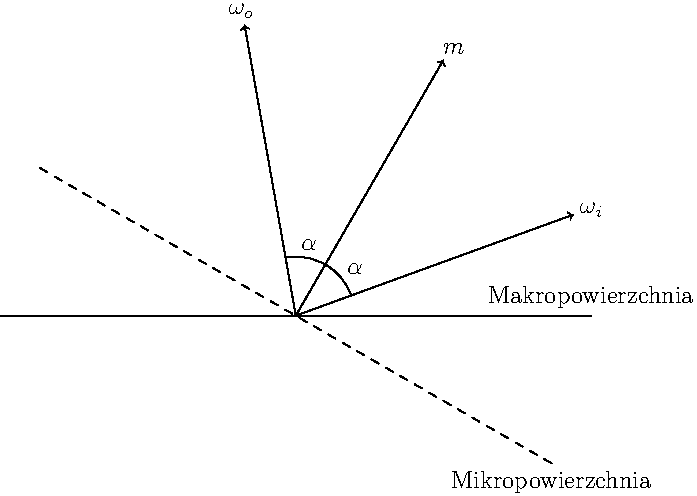
\includegraphics{montecarlo/ggx_sample_m}
    \caption{Wygenerowany wektor $m$ jest normalną mikropowierzchni, którą wykorzystujemy do obliczenia faktycznego kierunku światła przychodzącego. Opracowanie własne.}
    \label{fig:GGXSampleMReflect}
\end{figure}

\section{Monte-Carlo z wieloma funkcjami ważności}
\label{Chapter:MIS}

Załóżmy, że mamy $n$ różnych funkcji gęstości prawodpodobieństwa $p_{i}(x)$ dla $i \in \{ 1, \ldots, n \}$ opisujących istotność poszczególnych próbek dla danych czynników szukanej funkcji $f(x)$. Każda z tych strategii działa lepiej w pewnych obszarach dziedziny, jednakże gorzej od nich w każdym innym miesjcu. Chcielibyśmy dynamicznie wybierać, której strategii używać w danym momencie, tak aby wariancja spadła jeszcze bardziej.

Przykładem zastosowania tej metody jest równanie renderingu:
\[
L_o(\omega_o) = \int_{\Omega} {
	L_i(\omega_{i})
	f_r(\omega_{i}, \omega_{o})
	\cos \theta_{i}
	\dd\omega_{i}
}
\]

Jedną ze strategii modelowania jest modelowanie funkcji $f_r$, jednak nie zawsze kierunki istotne dla BRDF będą pokrywać się z kierunkami z których przychodzi światło tzn. $L_i$. Najlepszą strategią, byłoby generowanie kierunków istotnych z punktu widzenia $f_r$ oraz $L_i$. Dla większości materii nie będzie to tak istotne, jednak jeżeli zaczniemy rozpatywać powierzchnie lustrzane z niewielkim pojedyńczym źródłem światła w otoczeniu problem stanie się oczywisty: większość próbek wygenerowanych na podstawie BRDF będzie posiadała $L_i(\omega_i) \approx 0$. Podobnie dla strategii generowania próbek z $L_i$, dla większości kierunków $f_r(\omega_i) \approx 0$.

W takich sytuacjach właśnie znajduje zastosowanie technika Monte-Carlo z wykorzystaniem wielu funkcji ważności (ang. \textit{Multiple Importance Sampling}, \textit{MIS}).

W tej pracy technika ta nie będzie wykorzystywana do generowania obrazu w spośób bezpośredni, jednak jest ona nieoceniona przy dopasowywaniu parametrów aproksymacji.

Naiwnym podejściem do tego problemu jest obliczenie całki korzystając z każdej ze strategii i uśrednienie wyniku uzyskanego przez każdą z nich. Po dłuższym zastanowieniu widać jednak, że takie podejście nie da nam pożądanego rezultatu, wariancja nie spadnie ponieważ zmienne losowe są niezależne i wariancja końcowa będzie sumą wariancji poszczególnych strategii.

Zbudujemy więc model wielopróbkowy (ang. \textit{multi-sample model}) \cite{pbrt,ImportanceSamplingForProduction} korzystający z wygenerowanych próbek z wielu źródeł jednocześnie, których wyniki będą mieszane zgodnie z pewną rodziną funkcji ważących $w_i$. Nasz estymator Monte-Carlo funkcji $f$ w takiej sytuacji będzie wyglądał następująco:
\[
  F = \sum_{i=1}^{n} \frac{1}{n_i} \sum_{j=1}^{n_i} w_{i}(X_{i,j}) \frac{
    f(X_{i,j})
  }{
    p_{i}(X_{i,j})
  }
\]
\noindent gdzie:
\begin{itemize}
	\item $n$ - ilość strategii próbkowania,
	\item $n_i$ - ilość próbek wygenerowanych przez $i$-tą strategię,
	\item $w_i$ - funkcja wagi dla $i$-tej strategii próbkowania,
	\item $X_{i,j}$ - $j$-ta próbka wygenerowana przez $i$-tą strategię,
	\item $p_i$ - funkcja gęstości prawdopodobieństwa $i$-tej strategii.
\end{itemize}

% Źródło: MIS p.261
Aby estymator $F$ pozostał nieobciążony (ang. \textit{unbiased}) funkcja $w_i$ musi spełniać następujące warunki:
\[ \sum_{i = 1}^{n} w_{i}(x) = 1 \text{ dla } f(x) \neq 0 \]
\[
  \forall i \in \{ 1, \ldots, n \} \quad
  w_{i}(x) = 0 \Leftrightarrow p_i(x) = 0
\]

Za najlepszy wybór funkcji mieszającej $w_i$ sprawdzającej się w większości zastosowań uważa się funkcję postaci:
\[
  w_{i}(x) = \frac{
    n_{i} p_{i}(x)
  }{
    \sum_{k=1}^{n} {
      n_{k} p_{k}(x)
    }
  }
\]

% pbrt p799
\noindent biorącą pod uwagę wszystkie sposoby generacji próbki nazywaną heurystyką bilansującą (ang. \textit{balance heuristics}). Istnieje również kwadratowa heurystyka bilansująca \cite{pbrt}, która w praktyce bardzo często sprawdza się jeszcze lepiej \cite{pbrt,Veach}:
\[
  w_{i}(x) = 
  \frac{
	\left( n_{i} p_{i}(x) \right)^{\beta}
  }{
	\sum_{k=1}^{n} {
		\left(n_{k} p_{k}(x)\right)^{\beta}
	}
  }
\]

Z doświadczeń \cite{Veach} wynika, że wartość $\beta = 2$ jest bardzo dobrym wyborem.

\end{document}
